 \chapter{Appendix}
                \section{Probability and State Estimation}
                    \subsection{Probability Primer}
                        The study of the Theory of Probability could be described as the study of "uncertain outcomes" and it is easily one of the most counterintuitive fields of mathematics. It is also enormous. Here, only the very basics will be introduced, just enough to better understand the following discussions on \textit{Probabilistic Robotics} and \textit{Filters}. The following discussion will be pretty mathematically heavy and precise, but there will also be some colloquial paraphrasing of the introduced notions.
                        \subsubsection{Measurable Spaces and Probability Spaces}
                            \begin{definition}\label{sigma_algebra}
                                Let $\mathcal{F}$ be a non-empty family of subsets of a set $\Omega$. $\mathcal{F}$ is a $\sigma$\textit{-algebra} over $\Omega$ if and only if:
                                \begin{itemize}
                                    \item If $A \in \mathcal{F}$, then $A^c:=\Omega/A\in\mathcal{F}$: the set $\mathcal{F}$ is closed under taking complements.
                                    \item The countable \footnote{A set $X$ is \textit{countable} if and only if there exists a surjective mapping $f:\mathbb{N}\rightarrow X$} union of elements of $\mathcal{F}$ is still in $\mathcal{F}$: the set $\mathcal{F}$ is closed under taking the countable union of its elements.
                                \end{itemize}
                            \end{definition}
                            It is an easy exercise that a $\sigma$-algebra is also closed under countable intersections. Another two definitions, then the "why should we care" will be explained:
                            \begin{definition}\label{measurable_space}
                                A \textit{measurable space} is the couple $\left(\mathcal{F},\Omega\right)$ such that:
                                \begin{itemize}
                                    \item $\Omega\neq\emptyset$.
                                    \item $\mathcal{F}$ is a $\sigma$-algebra on $\Omega$.
                                \end{itemize}
                            \end{definition}
                            \begin{definition}\label{measure}
                                A \textit{measure} over the measurable space $\left(\mathcal{F},\Omega\right)$ is a function:
                                \begin{equation*}
                                    \mu:\mathcal{F} \rightarrow [0,+\infty]
                                \end{equation*}
                                Such that:
                                \begin{itemize}
                                    \item $\mu(\emptyset)=0$.
                                    \item $\mu$ is $\sigma$\textit{-additive} over $\mathcal{F}$, meaning that:
                                    \begin{equation*}
                                        \mu\left(\bigcup_{n=1}^{\infty}A_n\right)=\sum_{n=1}^{\infty}\mu(A_n)
                                    \end{equation*}
                                \end{itemize}
                            \end{definition}
                            The definition of $\sigma$-algebra is necessary in this context to represent \textit{events}: these are the measured result of a probabilistic experiment. However, events could also be composed of single \textit{outcomes}, which are represented by the elements of $\Omega$. As an example, in the experiment:
                            \begin{equation*}
                                \textit{If a dice is thrown, what is the probability of obtaining 5 as a result?}
                            \end{equation*}
                            The event $A$=\textit{"The result of the throw is 5"}$\in\mathcal{F}$ coincides with the outcome:
                            \[\omega_1=\textit{"the throw results in 5"}\in\Omega\]
                            However, it is equally plausible to ask:
                            \begin{equation*}
                                \textit{If a dice is thrown, what is the probability of obtaining a result smaller than 5?}
                            \end{equation*}
                            The event:
                            \[A=\textit{"The result of the throw is less than 5"}\in\mathcal{F}\]
                            Would actually be composed of more than one outcome: $A=\{\omega_1,\omega_2,\omega_3,\omega_4\}$. Then, the need for the definition of a measure is easily understood: it measures exactly the probability of the event passed to it as an argument. From these observations, the following definition is natural.
                            \begin{definition}
                                A measurable space $(\mathcal{F},\Omega,P)$ with $P(\Omega)=1$ is called a \textit{Probability Space}. The set $\Omega$ is called the \textit{set of outcomes}, $\mathcal{F}$ is the $\sigma$-algebra of \textit{events} and $P(A)$ is the \textit{probability} of the event $A\in\mathcal{F}$.   
                            \end{definition}
                            The requirement $P(\Omega)=1$ is obvious: it just states that \textit{some event} will surely manifest. Notice that the event $A=\Omega/\Omega=\emptyset\in\mathcal{F}$ is legal by the definition of $\sigma$-algebra, meaning that an event doesn't necessarily mean that \textit{something} will happen. 
                    \subsection{State Estimation: Filters}
                        One of the many differences between static robots and moving ones is the increased difficulty in state estimation. Indeed, an industrial manipulator has the possibility of using fixed landmarks and \textit{proprioceptive} sensors to estimate its state; meanwhile, for a mobile robot, this is not possible with high enough accuracy, due to the (often) dynamic environment and the additional noise afflicting the on the onboard sensors. The problem of \textit{State Estimation} is then solved by \textit{probabilistic} methods, in particular by making use of \textit{filters}.\\
                        Although a full discussion on filters would probably take an entire book, it is instructive to at least mention some of them and their differentiation. Filters can be divided into two main categories:
                        \begin{itemize}
                            \item \textit{Parametric Filters}: these assume a predefined formulation of the probability distribution for the state (probabilistic) variable $x$; often a Uniform Gaussian Distribution is assumed. These filters are capable of estimating the \textit{parameters} which describe the PDF\footnote{\textit{Probability Distribution Function}}. This kind of filters are very computationally efficient, however greatly sensitive to the system high nonlinearity and to multimodal distribution.
                            \item \textit{Non-Parametric Filters}: these don't assume \textit{any} kind of formulation for the PDF, but represent it by taking a set of samples, called \textit{particles}, and making computation based on them. These filters are called \textit{Particle Filters}. Although computationally heavy, they can represent a wide variety of PDFs, even multimodal ones.
                        \end{itemize}
                        \subsubsection{Parametric Filters}
                            There are plenty of types of parametric filters, but arguably the most famous is the \textit{Kalman Filter}. The Kalman Filter is a \textit{linear} (it assumes that the analyzed system's dynamics is linear) \textit{Gaussian} filter, i.e. it assumes that the state transition probability is a Gaussian PDF:
                            \begin{equation}\label{Gaussian_PDF}
                                p(x_t\mid u_t,x_{t-1})=\det(2\pi R_t)^{-1/2}exp\left\{-\frac{1}{2}\left(x_t-A_tx_{t-1}-B_{t}u_{t}\right)^{T}R_t^{-1}\left(x_t-A_tx_{t-1}-B_{t}u_{t}\right)\right\}
                            \end{equation}
                            Where:
                            \begin{itemize}
                                \item $x_t=A_tx_{t-1}+B_tu_t+\epsilon_t$ is the perturbed linear dynamic model of the system ($\epsilon_t$ is Gaussian noise).
                                \item $R_t$
                            \end{itemize}


                            
                \section{Motion Planning}
                    \subsection{Introduction}
                        A fundamental need in robotics is to have algorithms that convert high-level specifications of tasks from humans into low-level descriptions of how to move in an environment which can be either dynamic or static. A classic example of this is the \textit{Piano Mover's Problem}.
                        \begin{figure}[h!]
                            \centering
                            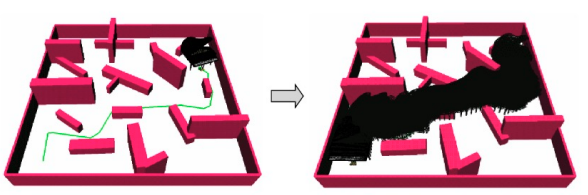
\includegraphics[width=0.8\linewidth]{Images/image22.png}
                            \caption{3D Piano Mover's Problem}
                            \label{fig:Piano_Movers_Problem}
                        \end{figure}
                        This need is expressed by the \textit{Motion Planning Problem}:
                        \begin{definition}\label{Motion_Planning_Problem}
                            Given the initial $q_0$ desired $q_d$ poses of a robot $\mathcal{B}$ in the environment $\mathcal{W}=\mathbb{R}^n$,$n\in\{2,3\}$, the problem of \textit{ Motion Planning} is to find, if it exists, a path that drives the robot between the two poses without any contact or collision with obstacles $\left\{\mathcal{O_{i}}\right\}_{i=1}^{p}$.
                        \end{definition}
                        Planning can be either done in \textit{online} during execution of the tasks, or \textit{offline}. Offline planning is obviously only really feasible if the environment does not change, i.e. it is \textit{static}. \\
                        Some assumptions are introduced:
                        \begin{itemize}
                            \item The positions of the obstacles $\{\mathcal{O_i}\}_{i=1}^{p}$ are known and fixed, at least for offline planning. Each set $\mathcal{O}_i$ is closed and contains its boundary. Notice that it is not necessary for the obstacles to be limited subsets of $\mathcal{W}$.
                            \item The robot $\mathcal{B}$ can move instantaneously everywhere (although this assumption will be relaxed later).
                        \end{itemize}
                    \subsection{Distance, Obstacles and \textit{Free Configuration Space}}
                        It is known that, on an Euclidean Space there always exists a metric (\textit{Euclidean Metric}) which in turn establishes a norm. However, the Configuration Space is not necessarily an Euclidean Space, which immediately begs the question of how to measure distances. Intuition suggests that the distance between two robot configurations, $q_1,q_2$, should be zero if the space occupied by the robot $\mathcal{B}$ in those configurations is the same; let:
                        \begin{itemize}
                            \item $\mathcal{B(q)}\subseteq\mathcal{W}$ be the subset of the environment occupied by the robot in the configuration $q$.
                            \item Let $p(q)$ be the position in $\mathcal{W}$ of a robot's point, taken as a reference. This naturally implies that $p\in\mathcal{B}$.
                        \end{itemize}
                        Then, the \textit{uniform metric} is adopted:
                        \begin{equation}\label{uniform_C_space_norm}
                            d(q_1,q_2)=\max_{p\in\mathcal{B}} ||p(q_1)-p(q_2)||
                        \end{equation}
                        Next, it is necessary to map an obstacle from $\mathcal{W}$ to the $\mathcal{C}$-space. This is done by introducing the \textit{C-obstacle}.
                        \begin{definition}
                            Let $\mathcal{O}_{i}\in\mathcal{W}$, $i \in \{1,\dots,p\}$, be an obstacle in $\mathcal{W}$. Then, the image of the obstacle in the configuration space is defined as:
                            \begin{equation}\label{C_obstacle_image}
                                \mathcal{CO}_{i}=\left\{q \in \mathcal{C}: \mathcal{B}(q) \cap \mathcal{O}_{i} \neq \emptyset \right\}
                            \end{equation}
                            This is the set of configurations that cause a collision with the $i$-th obstacle. Then, the union:
                            \begin{equation}\label{C_osbstacle}
                                \mathcal{CO}=\bigcup_{i=1}^{p}\mathcal{CO}_{i}
                            \end{equation}
                            It is called $\mathcal{C}$\textit{- obstacle region} and is the set of configurations that cause a collision with at least one obstacle.
                        \end{definition}
                        The complement of the $\mathcal{C}$-space with respect to $\mathcal{CO}$ gives:
                        \begin{definition}\label{free_configuration_space}
                            The \textit{Free Configuration Space} $\mathcal{C}_{free}$:
                            \begin{equation}\label{free_configuration_eq}
                                \mathcal{C}_{free}=\mathcal{C}/\mathcal{CO}
                            \end{equation}
                            Is the set of configurations which do not cause collisions with any obstacle. A \textit{free-path} is a path completely contained in $\mathcal{C}_{free}$
                        \end{definition}
                        The computation of these spaces is computationally heavy, if not outright intractable. However, it is possible to approximate them by \textit{sampling} the space and adopting \textit{Grid Representations}.
                    \subsection{Grid-Based Mapping}
                        The approximation of the $\mathcal{C}$-space is almost mandatory in real applications, as is easily understood. A structure used to represent the approximation of the $\mathcal{C}_{free}$ is called a \textit{Roadmap}. The most basic procedure adopted for an approximation-based Motion Planner could be:
                        \begin{itemize}
                            \item Approximate $\mathcal{C}_{free}$.
                            \item Find a path connecting $q_i$ to $q_f$, if it exists.
                            \item At each planner iteration, a sampled model configuration is chosen and checked if it leads to collisions with obstacles. if there are, the sample is discarded from $\mathcal{C}_{free}$; if there is no collision, the sample is saved in the current Roadmap.
                        \end{itemize}
                        \begin{figure}[htbp!]
                            \begin{minipage}{0.6\textwidth}
                                    \centering
                                    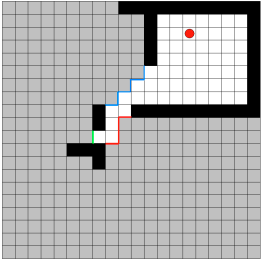
\includegraphics[width=0.6\linewidth]{Images/image23.png}
                                    \caption{Grid-Map}
                                    \label{fig:grid_map}
                            \end{minipage}\hfill
                            \begin{minipage}{0.4\textwidth}
                                A \textit{Grid-based} approximation is based on a discretization of the configuration space as a set of occupied and free cells; this approach can also be used in a $3D$ map. Increasing the resolution of the cells help to speed up the planning process, however giving rise to worse paths. This approach also has some criticalities which must be addressed in the design of the Motion Planner. In particular, the choice of an appropriate data structure is of great importance; a chosen data structure should be easy to read, maintain in memory and visualize for a human operator.
                            \end{minipage} 
                        \end{figure}
                        \subsubsection{Probabilistic Roadmap Method: \textit{PRM}}
                            Assuming to have successfully generated a grid-map, it is then time to plan a motion. The most n\"{a}ive approach would be to (uniformly) randomly generate a sample configuration $q_s\in \mathcal{C}$ and check its feasibility, either by a direct representation of $\mathcal{CO}$ or by kinematics arguments. \\
                            The procedure at $i$-th iteration would look like:
                            \begin{itemize}
                                \item Generate the random sample $q_s^{(i)}$.
                                \begin{itemize}
                                    \item If $q_s^{(i)}$ generates a collision, it is discarded.
                                    \item if $q_s^{(i)}$ does not generate a collision, it is added to the Roadmap.
                                \end{itemize}
                                \item The \textit{Local Planner} checks for the nearest feasible configuration $q_{near}^{(i)}$, based on the used metric on $\mathcal{C}$. A path is searched to link $q_s^{(i)}$ and $q_{near}^{(i)}$. A common choice of such a path would be a rectilinear path, which is sampled and checked for collision.
                            \end{itemize}
                            Once the iterations stop (due to some criterion), a representation of $\mathcal{C}_{free}$ is obtained. The next step is to find paths that connect $q_i$, $q_f$ completely contained into $\mathcal{C}_{free}$. Then:
                            \begin{itemize}
                                \item The Local Planner links $q_s$ and $q_f$ to the Roadmap.
                                \item A search algorithm is used to find the path connecting $q_s,q_f$ along the Roadmap.
                            \end{itemize}
                            Notice that the PRM is probabilistic, which means that if a solution that connects the initial and desired configurations does not exist, the algorithm keeps on searching without ever stopping. However, it has the advantage of not requiring an explicit description of $\mathcal{CO}$, which is a big deal. 
                        \subsubsection{Artifical Potential Methods}
                            Although powerful, PRM has been used under the assumption of a static environment. However, it often the case that robots have to execute tasks in a \textit{dynamic} environment. To this end, the method of \textit{Artificial Potential} is introduced; its main objective is not to reconstruct $\mathcal{C}_{free}$, but only to reach the desired configuration $q_f$.\\
                            The method exploits the superposition of two terms:
                            \begin{itemize}
                                \item An \textit{attractive} potential term, which guides the robot:
                                    \begin{itemize}
                                        \item A first choice could be:
                                            \begin{equation}\label{attractive_potentia_1}
                                                U_a(q)=\frac{1}{2}k_ae^{T}(q)e(q)=\frac{1}{2}k_a ||e(q)||^2
                                            \end{equation}
                                            Where $k_a>0, e(q)=q_f-q$. The resulting force is:
                                            \begin{equation*}
                                                f_a(q)=-\nabla U_a(q)=k_a e(q)
                                            \end{equation*}
                                        \item Another choice could be:
                                            \begin{equation}\label{attractive_potential_2}
                                                U_b(q)=k_a||e(q)||
                                            \end{equation}
                                            Where $k_a>0,e(q)=q_f-q$. The resulting force is:
                                            \begin{equation*}
                                                f_b(q)=-\nabla U_b(q)=k_a \frac{e(q)}{||e(q)||}
                                            \end{equation*}
                                            However note that this is not defined at the target configuration and the robot converges more slowly to the target than with the other choice. However, this force doesn't go to infinity for large errors $e(q)$, so it is useful for starting configurations.
                                    \end{itemize}
                                \item A \textit{repulsive} potential term, which pushes the robot away from the $\mathcal{CO}-$obstacle region. Assuming $\mathcal{CO}$ to be convex or partitioned into convex regions $\mathcal{CO}_i$, then each region's associated repulsive potential is:
                                \begin{equation}\label{repulsive_potential}
                                    U_{r,i}(q)=
                                    \begin{cases}
                                        \frac{k_{r,i}}{\gamma} \left[\frac{1}{\eta_i(q)}-\frac{1}{\eta_{o,i}(q)}\right]^\gamma \text{, } \eta_i(q)\leq \eta_{o,i} \\
                                        0 \text{, } \eta_{i}(q)>\eta_{o,i}
                                    \end{cases}
                                \end{equation}
                                Where: 
                                \begin{itemize}
                                    \item $k_{r,i}>0$ is a positive gain.
                                    \item $\eta_i(q)=\min_{q'\in \mathcal{CO}_{i}}||q-q'||$.
                                    \item $\eta_{o,i}$ is the obstacle's \textit{range of influence}.
                                    \item $\gamma \in \{2,3\}$.
                                \end{itemize}
                                Then, the induced force is:
                                \begin{gather*}
                                    f_{r,i}(q)=- \nabla U_{r,i}(q)= \\
                                    \begin{cases}
                                        \frac{k_{r,i}}{\eta_{i}^{2}(q)} \left[\frac{1}{\eta_{i}(q)}-\frac{1}{\eta_{o,i}}\right]^{\gamma-1} \nabla\eta_i(q), \text{ }\eta_i(q) \leq \eta_{o,i} \\
                                        0, \text{ } \eta_i(q)>\eta_{o,i}
                                    \end{cases}
                                \end{gather*}
                                The convexity hypothesis was necessary for $\nabla \eta_i(q)$ to be analytically computed.
                            \end{itemize}
                            The total potential and force are then the sum of all individual potentials and forces. Although the name suggests it, the total force is \textit{not} necessarily applied as an actual force on the robot, in fact there are different interpretations:
                            \begin{itemize}
                                \item $f_t(q)=\tau$: The total force is seen as the vector of generalized forces (force plus torques) that induce a motion of the robot according to its dynamic model. If the planning is online, the total force is taken as the input to the robot; otherwise, it generates smooth trajectories since the reactions of the robot are filtered by the robot dynamics.
                                \item $f_t(q)=\ddot{q}$: The total force is seen as the acceleration moving the robot, that is considered as a point mass. In the case of online planning, a solution of the inverse dynamics problem or an online $2$° order kinematic control scheme are required. 
                                \item $f_t(q)=\dot{q}$: The total force is seen as the velocity vector moving the robot, that is considered from a kinematic viewpoint only. This is the most common choice, with the unique advantage of ensuring the reachability of the final configuration $q_f$ with zero velocity (meanwhile the other control schemes require an additional damping term).
                            \end{itemize}
                            Notice that Artificial Potential Methods suffer from a drawback: local minima. These can cause the robot to stall in configurations different from the desired ones:
                            \begin{gather*}
                                \begin{cases}
                                    f_t(\bar{q})=0\\
                                    U_t(\bar{q})>0
                                \end{cases} \text{ with }\bar{q}\neq q_g
                            \end{gather*}
                            These are generally addressed by heuristic methods.
            \newpage
                \section{Lyapunov Theory}
                    \subsection{LaSalle's Invariant Set Theorem}
                    \subsection{Barbalat's Lemma}
                        Lyapunov's Theorem establishes that given a Lyapunov Function whose derivative is negative definite, at least in a local neighbor of the origin, then the origin is an asymptotically stable equilibrium. However, finding a Lyapunov Function is a laborious task, especially with the required negative-defineteness on its Lie Derivative. In the case of autonomous systems, i.e. systems with no explicit time dependence, it is possible to apply LaSalle's Invariant Set Theorem to prove asymptotical stability of the equilibrium, given a \textit{semi}-negative definite Lie Derivative of the Lyapunov Function; unfortunately, this does not work with \textit{non-autonomous} systems, which are of interest in the context of mobile robots. \\
                        This problem is addressed by another fundamental result in stability theory: \textit{Barbalat's Lemma}. There are a few formulations of this theorem, but the most used one is the following:
                        \begin{definition}
                            (\textit{Barbalat's Lemma in scalar form} ($1$)): Let $f(t): \mathbb{R}\rightarrow\mathbb{R}$ have a finite limit for $t\rightarrow\infty$ and $\dot{f}(t)$ uniformly continuous; then, $\dot{f}(t)\rightarrow0$ for $t\rightarrow\infty$. 
                        \end{definition}
                        Notice that $|\ddot{f}(t)|<\infty$ is a sufficient condition for $\dot{f}(t)$ to be uniformly continuous. There is also an alternative version:
                        \begin{definition}
                            (\textit{Barbalat's Lemma in scalar form} ($2$)): Let $p\in[1,\infty)$, $q\in(1,\infty]$. If $f\in\mathcal{L}^{p}(0,\infty)$
                            \footnote{Remember that a function $f$ is an element of $\mathcal{L}^{p}(a,b)$ if and only if: 
                            \begin{equation*}
                                \left[\int_{a}^{b}{|f(x)|^{p}dx}\right]^{p}<\infty
                            \end{equation*}
                            } 
                            and $\dot{f}\in \mathcal{L}^{q}(0,\infty)$, then $f(t)\rightarrow0$ as $t\rightarrow\infty$.
                        \end{definition}
                        In vector form the theorem becomes:
                        \begin{definition}
                            (\textit{Barbalat's Lemma in vector form}): Let $f(t): \mathbb{R}^{n}\rightarrow\mathbb{R}^{m}$ be uniformly continuous over the Banach Space $(E,||\cdot ||)$\footnote{Remember that a Banach Space is an normed space $(E,||\cdot ||)$ closed under Cauchy sequences.} and assume:
                            \begin{equation*}
                                \lim_{t\rightarrow \infty}\left|\int_{0}^{t}{f(\tau)d\tau}\right| <\infty
                            \end{equation*}
                            Then, $f(t)\rightarrow0$ as $t\rightarrow\infty$.
                        \end{definition}
            \newpage
                \section{Mathematical Appendix}
                    \subsection{Vector Fields and Operators}
                        \begin{definition}
                        (\textit{Vector Field}): Given a subset $S\subseteq \mathbb{R}^{n}$, a \textit{vector field} is represented by a vector-valued function $V: S \rightarrow \mathbb{R}^{n}$ in standard Cartesian Coordinates. 
                        \end{definition}
                        If each component of $V$ is continuous, then $V$ is a continuous vector field. If each component is \textit{smooth} (meaning $C^\infty$), then so is the vector field. Geometrically speaking, a vector field assigns a vector to each point in space.
                        Similarly, a \textit{Co-vector Field} is a vector field acting on co-vectors. Since $f$ maps onto $\mathbb{R}^n$, it is possible to use the standard inner-product:
                        \[\langle w^*,v\rangle=\sum_{j}w_{j}^{*}v_j\]
                        There are other useful operators that will be needed from now on:
                        \begin{itemize}
                            \item \textit{Gradient}: This one should also be already familiar; assume $\lambda:\mathbb{R}^n \rightarrow \mathbb{R}$, the \textit{Gradient} of $\lambda$ is defined as:
                            \begin{equation}\label{Gradient}
                                d\lambda(x)=\left[\frac{\partial\lambda}{\partial x_1}, \dots,\frac{\partial\lambda}{\partial x_n}\right]
                            \end{equation}
                            \item \textit{Lie Derivative}: Let $f$ be a vector field and $\lambda$ a real-valued scalar function, then the \textit{Lie Derivative} is defined as:
                            \begin{equation}\label{Lie_Derivative}
                                L_{f}\lambda=\langle\lambda(x),f(x)\rangle=\frac{\partial\lambda}{\partial x}\cdot f(x)               
                            \end{equation}
                            Geometrically, it expresses how the vector field is oriented with respect to the gradient of the scalar field.
                            \item \textit{Lie Bracket}: Let $f,g$ be two vector fields; then the \textit{Lie Bracket} is defined as:                         \begin{equation}\label{Lie_Bracket}                                    \left[f(x),g(x)\right]=\frac{\partial g}{\partial x} f- \frac{\partial f}{\partial x} g 
                            \end{equation}
                            
                        \end{itemize}
                    \subsection{Distributions}
                        \definition{Distribution: Suppose that $\{f_i\}_{i=1}^{d}$ is a set of vector fields defined on the open set $U\subseteq\mathbb{R}^{n}$. Then, a \textit{Distribution} is:
                        \begin{equation}\label{Distribution}
                            \Delta(x)=span\left\{f_1(x),f_2(x),\dots,f_d(x)\right\}
                        \end{equation} 
                        A distribution is \textit{nonsingular} if $dim(\Delta(x))=d$, $\forall x \in U$.}
                        A point $x_0 \in U$ is said to be \textit{regular} if there is a neighborhood $U^0(x_0)\subseteq U$ such that $\Delta(x)$ is nonsingular over $U^0$.
                        \begin{lemma}\label{smoot_distributions}
                            Let $\Delta$ be a smooth distribution and $x_0$ be a regular point. Then, there exists an open neighborhood $U^0(x_0)$ of $x_0$ and a set of vector fields $\{f_i\}_{i=1}^{d}$ defined on $U^0(x_0)$, with the following properties:
                            \begin{itemize}
                                \item The vectors $\{f_i\}_{i=1}^{d}$ are linearly independent for all $x$ in $U^0$.
                                \item $\Delta(x)=span\left\{f_1,\dots,f_d\right\}$ at each $x$ in $U^0$.
                                \item Every smooth vector field $g \in \Delta$ can be expressed on $U^0$ as a linear combination of the vector fields $\{f_i\}_{i=1}^{d}$:
                                \begin{equation*}
                                    g=\sum_{i=1}^{d}c_i(x)f_i(x)
                                \end{equation*}
                                Where $\{c_i\}_{i=1}^{d}$ are smooth real-valued functions on $U^0$.
                            \end{itemize}
                        \end{lemma}
                        In Control Theory, and in particular in Control-Affine systems, it is often the case that a Feedback-Linearization is of interest to simplify and stabilize the system's dynamics. In linear systems, feedback linearization is easily achieved if the system is stabilizable and observable; however, in non-linear systems it is required to introduce another concept, that of \textit{Involutivity}.
                        \definition{\textit{Involutivity}: A distribution is \textit{involutive} if the Lie Bracket $[\tau_1,\tau_2]$ of any pair of vector fields $\tau_1,\tau_2 \in \Delta$ is a vector field in $\Delta$:
                        \begin{equation*}
                            [\tau_1,\tau_2]\in\Delta, \forall \tau_1,\tau_2 \in \Delta
                        \end{equation*}
                        By the previous lemma:
                        \[\tau_j=\sum_{i}c_i^jf_i\]
                        So that the distribution is involutive if and only if:
                        \begin{equation}\label{involutivity}
                            [f_i,f_j]\in\Delta, \forall f_i,f_j \in \Delta, 1\leq i,j\leq d
                        \end{equation}}
                        Notice that by definition any 1-dimensional distribution is involutive and that the zero vector belongs to any distribution by default. \\
                        It is often the case that one can generate a co-distribution from a given distribution or viceversa. 
                        \definition{\textit{Annhilator:} The \textit{Annhilator} of a distribution $\Delta$ is the co-distribution:
                       \begin{equation}\label{annhilator}
                            \Delta^{\perp}=\left\{w^*\in\mathbb{R}^{n^*}: \langle w^*,v\rangle=0, \forall v \in \Delta\right\}
                        \end{equation}
                        Notice that $\dim(\Delta)+\dim(\Delta^\perp)=n$
                        }